\documentclass[11pt]{article}
\usepackage{graphicx}
\usepackage{float}
\usepackage{hyperref}
\usepackage{natbib}
\usepackage{listings}
\usepackage{xcolor}
\usepackage[dvipsnames]{xcolor}
\usepackage[svgnames]{xcolor}
\usepackage{amsmath} % For the equation* environment
\usepackage{amssymb}

\hypersetup{
    colorlinks=true,
    linkcolor=red,
    filecolor=cyan,      
    urlcolor=orange,
    pdftitle={Overleaf Example},
    pdfpagemode=FullScreen,
    }

\setlength{\textwidth}{6.5in}
\setlength{\headheight}{0in}
\setlength{\textheight}{8.0in}
\setlength{\hoffset}{0in}
\setlength{\voffset}{0in}
\setlength{\oddsidemargin}{0in}
\setlength{\evensidemargin}{0in}

\lstdefinestyle{txtstyle}{
    basicstyle=\ttfamily\small,
    breaklines=true,
    backgroundcolor=\color{Bisque}
}
\lstset{style = txtstyle}

\definecolor{codegreen}{rgb}{0,0.6,0}
\definecolor{codegray}{rgb}{0.5,0.5,0.5}
\definecolor{codepurple}{rgb}{0.58,0,0.82}
\definecolor{backcolour}{rgb}{0.95,0.95,0.92}

\lstdefinestyle{mystyle}{
    backgroundcolor=\color{backcolour},   
    commentstyle=\color{codegreen},
    keywordstyle=\color{magenta},
    numberstyle=\tiny\color{codegray},
    stringstyle=\color{codepurple},
    basicstyle=\ttfamily\footnotesize,
    breakatwhitespace=false,         
    breaklines=true,                 
    captionpos=b,                    
    keepspaces=true,                                   
    numbersep=5pt,                  
    showspaces=false,                
    showstringspaces=false,
    showtabs=false,                  
    tabsize=2
}

\title{Computational Physics ps-4 Report}
  
\author{Tongzhou Wang, \\ GitHub account: TZW56203, repository: phys-ga2000, \\ \url{https://github.com/TZW56203/phys-ga2000}}

\date{September 30, 2024}

\begin{document}

\maketitle

\section{Problem 1}
\subsection{Part (a) and (b)}
Figure \ref{fig:C_v-T} shows the heat capacity as a function of temperature from $T$ = 5 K to $T$ = 500 K.
\begin{figure}[H]
    \centering
    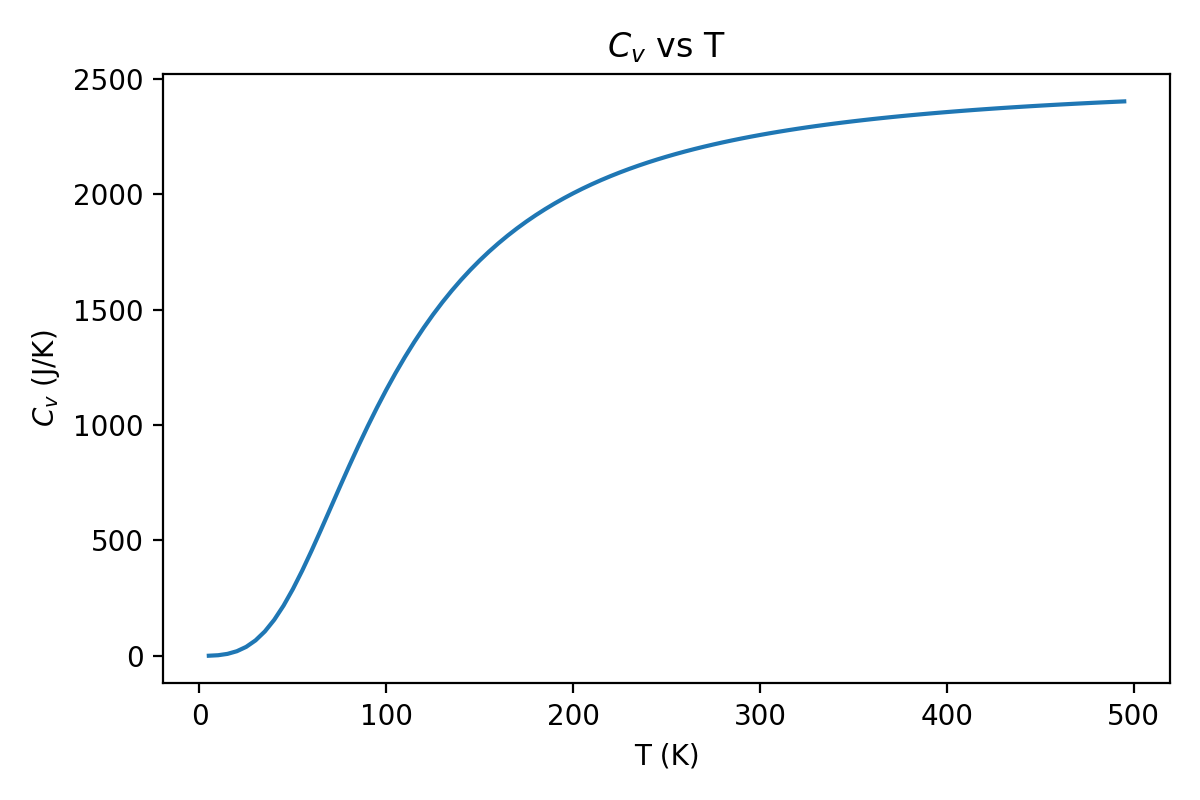
\includegraphics[scale = 1.0]{images/ps-4-1ab.png}
    \caption{Heat capacity vs temperature.}
    \label{fig:C_v-T}
\end{figure}

According to web sources, aluminum has specific heat capacity (at 298 K) 0.90 J $\mathrm{g^{-1}}$ $\mathrm{K^{-1}}$ and density 2.7 g/$\mathrm{cm^3}$. Our sample has volume 1000 $\mathrm{cm^3}$. Hence its heat capacity at 298 K should be
\begin{equation}
    0.90 \ \mathrm{J} \mathrm{g^{-1}} \mathrm{K^{-1}} \times 2.7 \ \mathrm{g}/ \mathrm{cm^3} \times 1000 \ \mathrm{cm^3} = 2430 \ \mathrm{J}/\mathrm{K}.
\end{equation}
This roughly agrees with the data in Figure \ref{fig:C_v-T}.

\subsection{Part (c)}
Figure \ref{fig:C_v-N_T298} and \ref{fig:C_v-N_T5} shows that our computation of $C_v$ converges. Specifically, in Figure \ref{fig:C_v-N_T5}, where $T$ = 5 K, we can see that $C_v$ converges as the number of points $N$ increases. This is reasonable as smaller $T$ implies larger integrating interval, which may require more points to accurately compute the integral.
\begin{figure}[H]
    \centering
    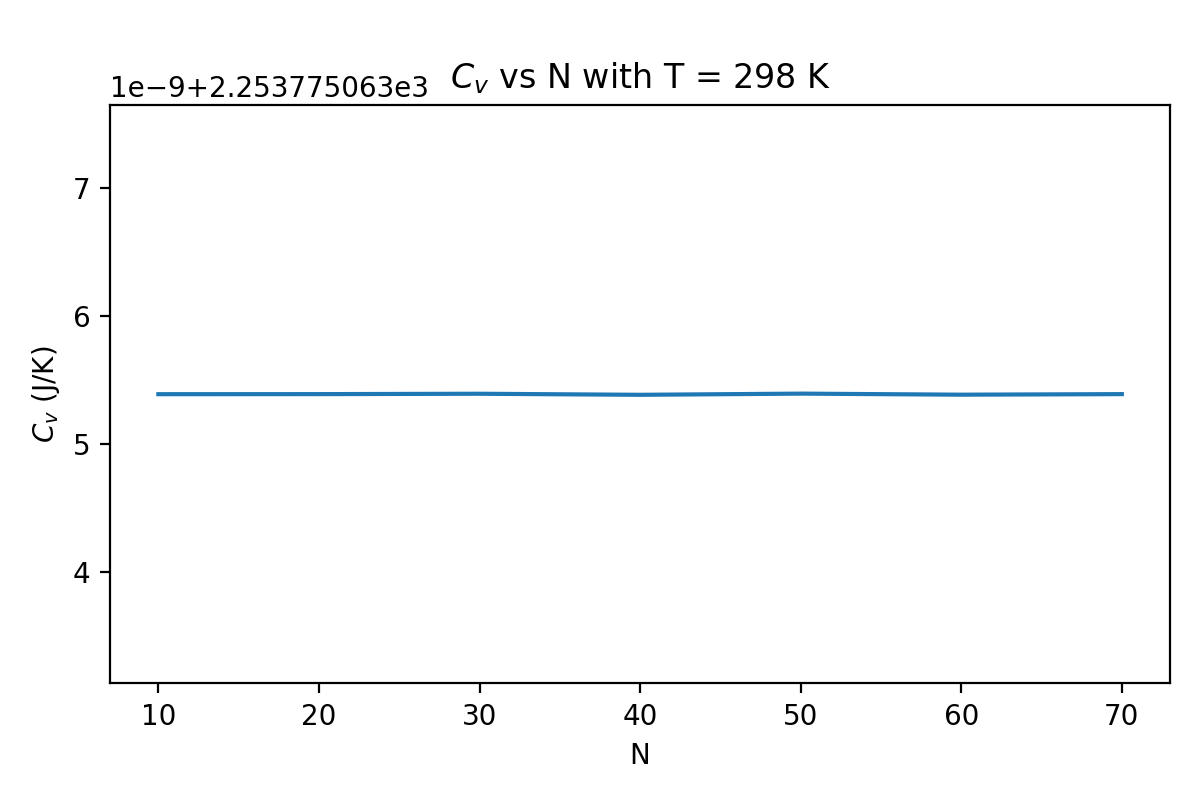
\includegraphics[scale = 1.0]{images/ps-4-1c_T298.png}
    \caption{$C_v$ vs $N$ with $T$ = 298 K.}
    \label{fig:C_v-N_T298}
\end{figure}
\begin{figure}[H]
    \centering
    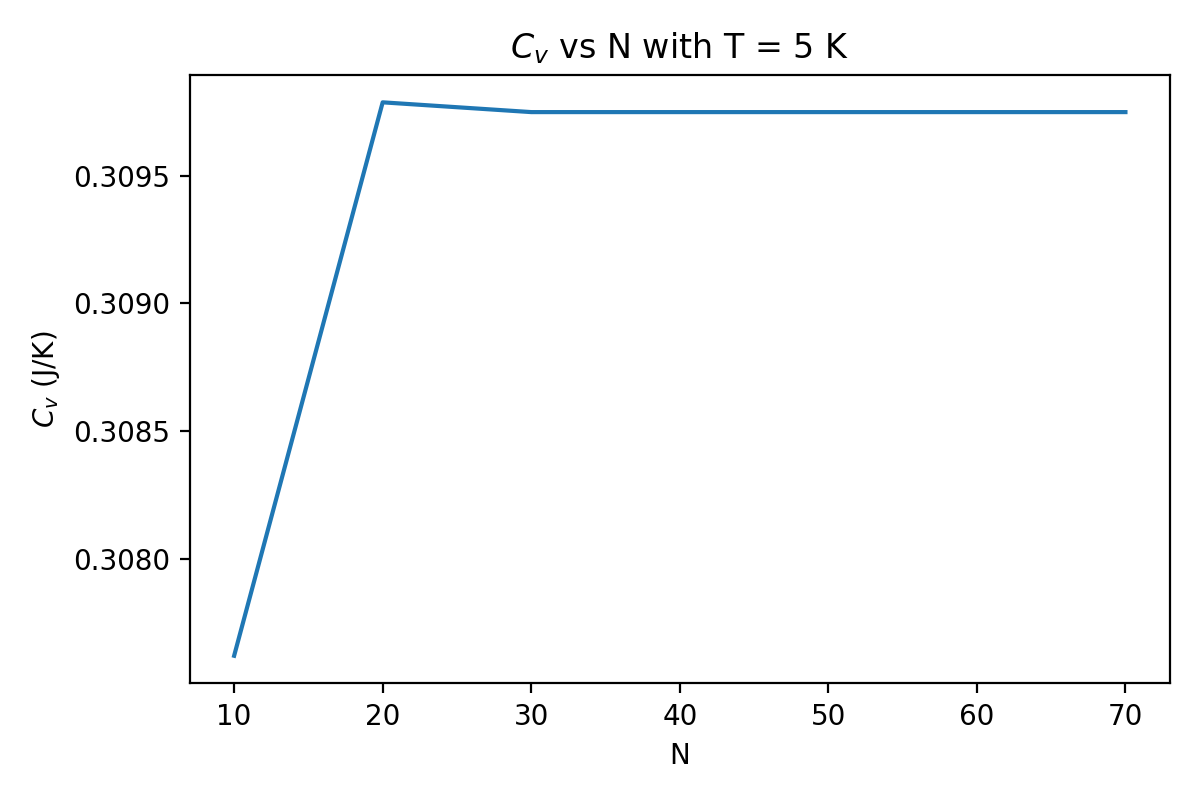
\includegraphics[scale = 1.0]{images/ps-4-1c_T5.png}
    \caption{$C_v$ vs $N$ with $T$ = 5 K.}
    \label{fig:C_v-N_T5}
\end{figure}

\section{Problem 2}
\subsection{Part (a)}
To begin with, we have
\begin{equation}
    \begin{cases}
        E = \frac{1}{2} m (\frac{dx}{dt})^2 + V(x), \\
        E = V(a).
    \end{cases}
\end{equation}
Rearranging, we have
\begin{equation}
    \frac{2[V(a) - V(x)]}{m} = (\frac{dx}{dt})^2,
\end{equation}
which becomes
\begin{equation}
    dt = \sqrt{\frac{m}{2[V(a) - V(s)]}} dx.
\end{equation}
Integrating, we have
\begin{equation}
    \int_0^{T/4} dt = \sqrt{\frac{m}{2}} \int_0^a \frac{dx}{\sqrt{V(a) - V(x)}}.
\end{equation}
Finally, we get
\begin{equation}
    T = \sqrt{8m} \int_0^a \frac{dx}{\sqrt{V(a) - V(x)}}.
\end{equation}

\subsection{Part (b)}
Figure \ref{fig:T-a} shows the period for amplitudes ranging from $a = 0$ to $a = 2$.
\begin{figure}[H]
    \centering
    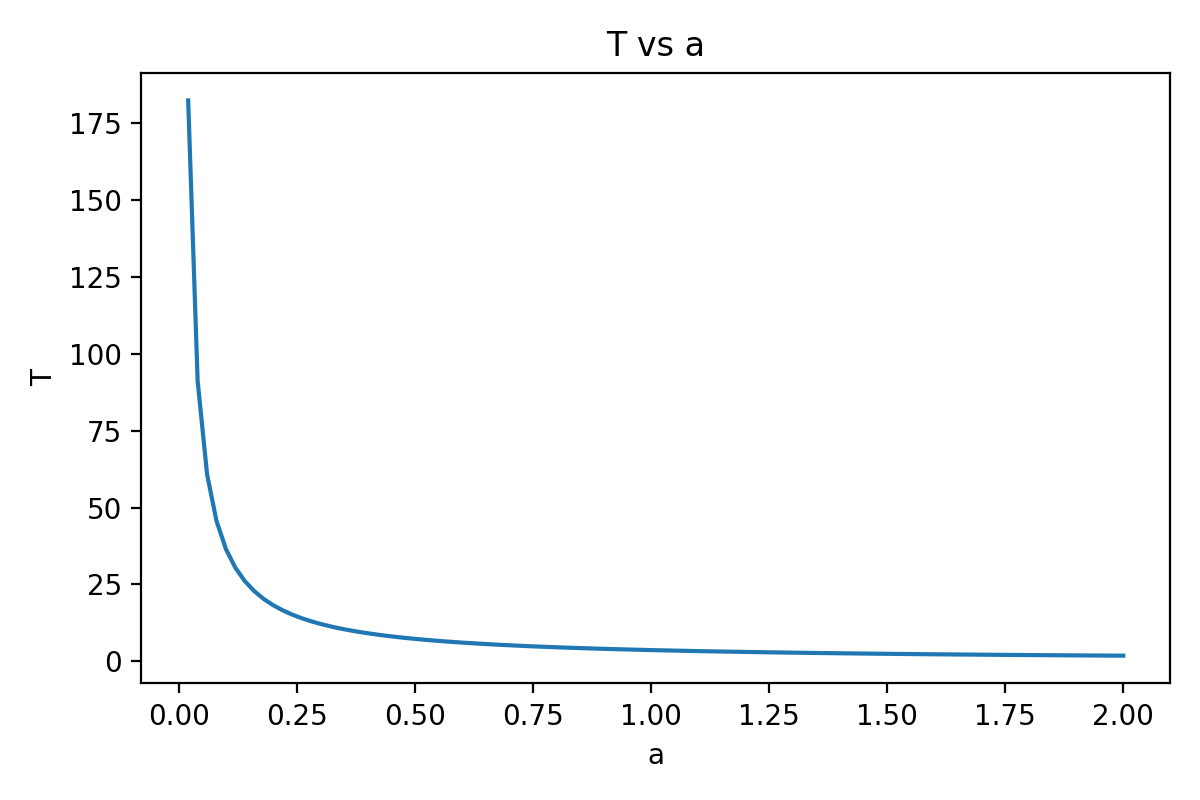
\includegraphics[scale = 1.0]{images/ps-4-2b.png}
    \caption{$T$ vs $a$.}
    \label{fig:T-a}
\end{figure}

\subsection{Part (c)}
Figure \ref{fig:T-a} shows that the period decreases as the amplitude increases, and the period diverges as the amplitude goes to zero. This can be explained by Figure \ref{fig:lnT-lna}, which shows that
\begin{equation}
    T \propto \frac{1}{a}.
\end{equation}
This can also be checked by analytically finding the integral
\begin{equation}
    \int_0^a \frac{dx}{\sqrt{a^4 - x^4}} =  \frac{\sqrt{\pi} \Gamma (5/4)}{a \Gamma (3/4)}.
\end{equation}
\begin{figure}[H]
    \centering
    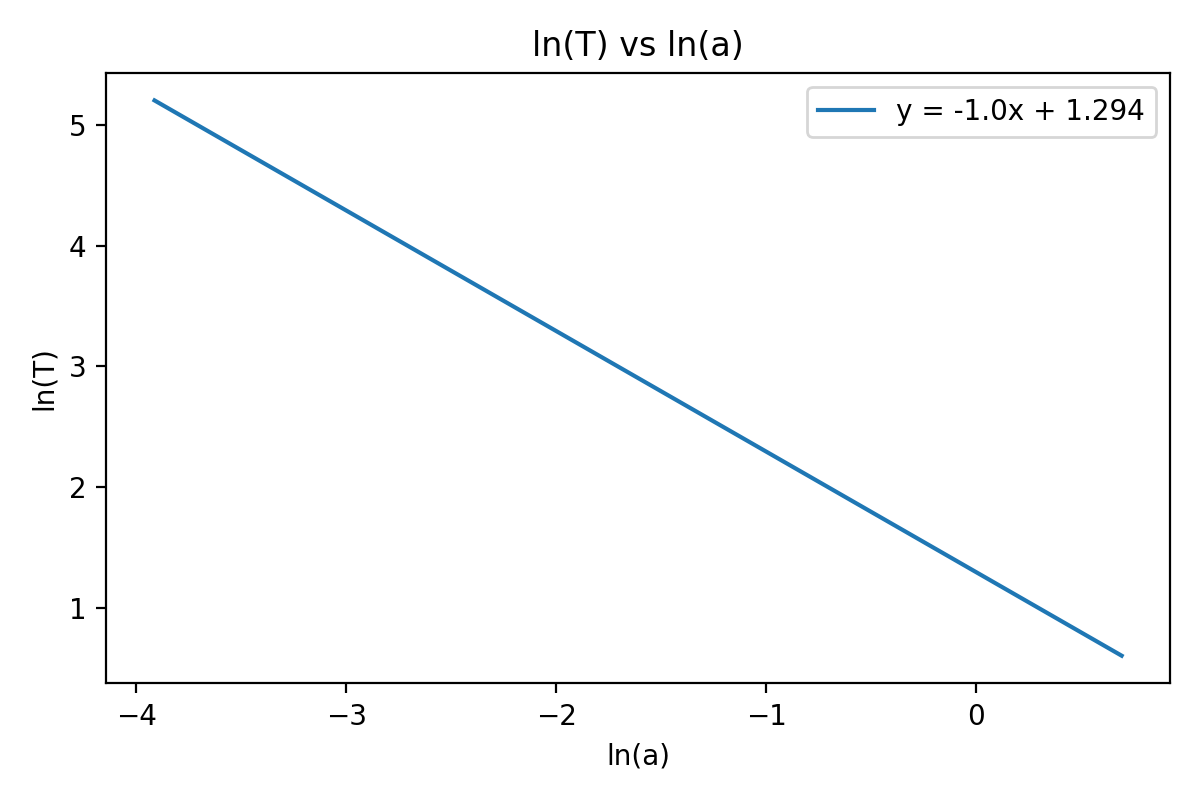
\includegraphics[scale = 1.0]{images/ps-4-2c.png}
    \caption{$\ln{(T)}$ vs $\ln{(a)}$.}
    \label{fig:lnT-lna}
\end{figure}

\section{Problem 3}
\subsection{Part (a) and (b)}
\begin{figure}[H]
    \centering
    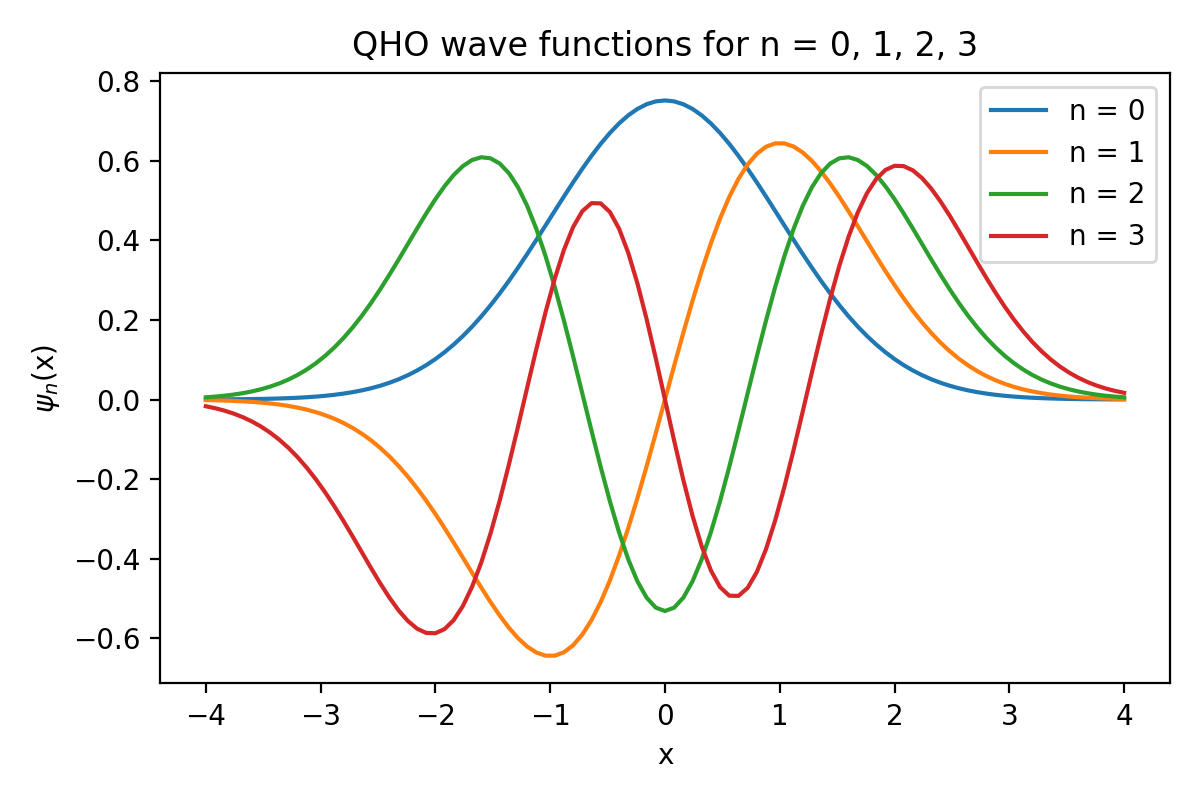
\includegraphics[scale = 1.0]{images/ps-4-3a.png}
    \caption{QHO wave functions for $n = 0, 1, 2, 3$.}
    \label{fig:QHO0123}
\end{figure}
\begin{figure}[H]
    \centering
    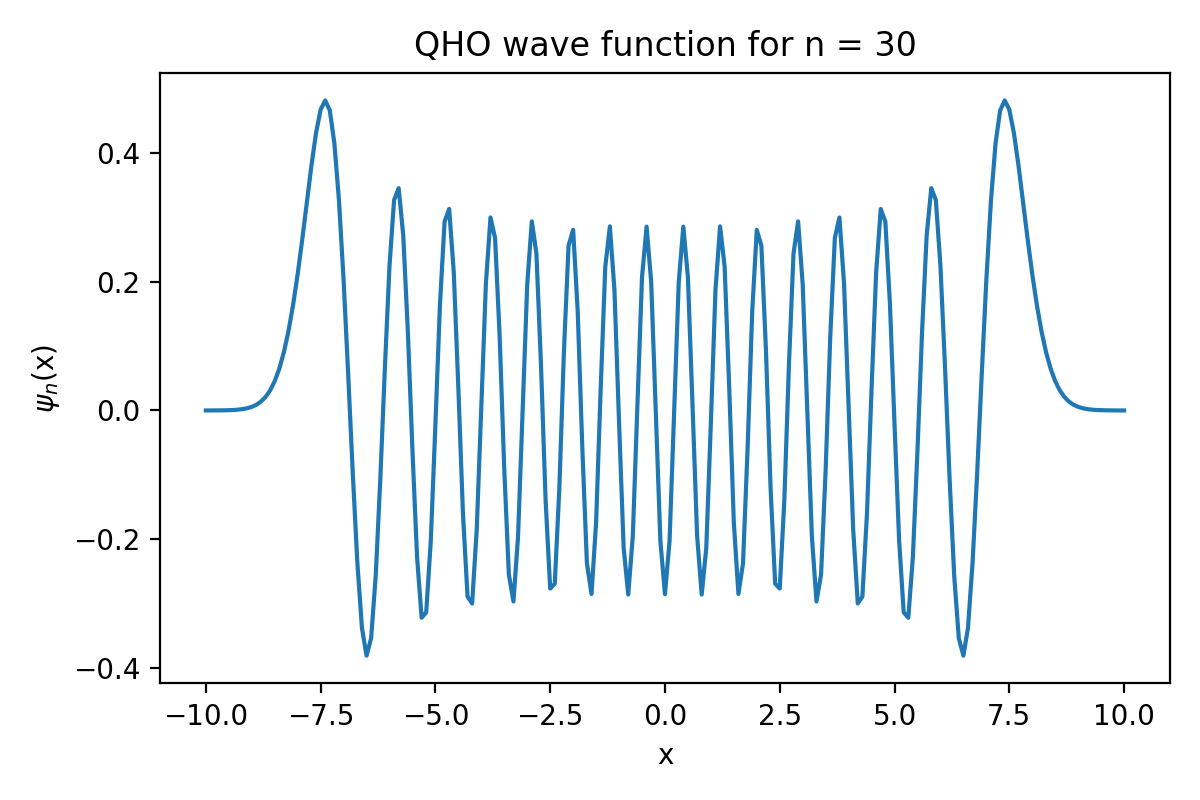
\includegraphics[scale = 1.0]{images/ps-4-3b.png}
    \caption{QHO wave functions for $n = 30$.}
    \label{fig:QHO30}
\end{figure}

\subsection{Part (c) and (d)}
Using Gauss-Hermite quadrature, we can make an exact evaluation of the integral. Note that for $n = 5$, the polynomial in the integrand should be of degree 12, so $N = 7$ sample points should be enough for the Gauss-Hermite quadrature to give zero approximation error. We did not choose larger $N$ here to avoid round-off errors.
\lstinputlisting[]{code/ps-4-3cd.txt}

\end{document}
